\documentclass[12pt,a4paper]{extreport}
\usepackage[italian]{babel}

\usepackage{geometry}
\usepackage{amsmath}

\usepackage{graphicx}
\usepackage{float}
% \usepackage{svg}
% \svgsetup{inkscapeexe="C:\Program Files\Inkscape\bin\inkscape.exe"}
% \svgpath{{immagini/}}
\graphicspath{{immagini/}}
\usepackage{xcolor}
\usepackage[colorlinks, linkcolor=blue, backref=section]{hyperref}


\begin{document}

%formattazione
\textwidth=450pt
\topmargin=-50pt
\textheight=675pt

%colori
\definecolor{letters}{HTML}{CECECE}
\definecolor{back}{HTML}{313030}
\definecolor{links}{HTML}{016AD3}
%\pagecolor{back}
%\color{letters}


%titolo
\begin{titlepage}
    \topmargin=-50pt
    \begin{center}
    {{\Large{\textsc{Alma Mater Studiorum $\cdot$ Universit\`a di
    Bologna}}}} \rule[0.1cm]{15.8cm}{0.1mm}
    \rule[0.5cm]{15.8cm}{0.6mm}
    {{\bf INGEGNERIA DELL’ENERGIA ELETTRICA E DELL’INFORMAZIONE 
    “GUGLIELMO MARCONI”\\
    \small CORSO DI LAUREA IN INGEGNERIA BIOMEDICA}}
    \end{center}
    \vspace{15mm}
    \begin{center}
    {\LARGE{\bf Energy Harvesting per}}\\
    \vspace{3mm}
    {\LARGE{\bf Dispositivi Indossabili}}\\
    \vspace{2cm}
    {\large{\bf Elaborato in Elettronica}}
    \end{center}
    \vspace{7cm}
    \par
    \noindent
    \begin{minipage}[t]{0.47\textwidth}
    {\large{\bf Relatore:\\
    Prof. Claudio Fiegna}}
    \end{minipage}
    \hfill
    \begin{minipage}[t]{0.47\textwidth}\raggedleft
    {\large{\bf Presentata da:\\
    Simone Morgagni}}
    \end{minipage}
    \vspace{20mm}
    \begin{center}
    {Anno Accademico 2023/2024}
    \end{center}
\end{titlepage}

\tableofcontents
\pagenumbering{arabic}

%body
\chapter{Introduzione}

\begin{section}{Dispositivi Indossabili}
    Pur essendo presenti in campo medico da tempo, i dispositivi indossabili e impiantabili hanno subito una rapida evoluzione. Tra le possibili applicazioni si hanno diagnosi attraverso la registrazione di segnali e marcatori biologici, ma anche terapia attraverso stimoli elettrici o rilascio di medicinali. In particolare la portabilita' abilita al funzionamento lontano dagli ospedali, rispondendo ai requisiti della telemedicina. Questo li rende particolarmente adatti al trattamento di condizioni croniche, sgravando sia strutture sanitarie, che pazienti. Permettono inoltre misure costanti, a lungo termine e non invasive. 

    I dispositivi indossabili, oltre a sensori e attuatori specifici per l'applicazione, richiedono anche componenti a bassa potenza come processori e antenne. Questi componenti sono necessari per svolgere funzioni di controllo automatico, elaborazione e trasmissione dei segnali misurati. Quando un modulo wireless e' disponibile, invece di conservare i dati, e' possibile inviarli a una hub intermedia o direttamente al destinatario finale in una struttura medica.

    La forma ideale e' piccola abbastanza da svolgere le funzioni volute senza intralciare il paziente. Nelle installazioni invasive e' essenziale che le dimensioni siano ridotte per abbassare i rischi e la complessita' dell'operazione. Anche nel caso non invasivo pero', si preferiscono dispositivi sottili e di piccole dimensioni che possono sostituire o integrarsi a capi di abbigliamento. L'aspetto non intrusivo o piacevole puo' incentivare l'uso regolare. Evitare dimenticanze e' infatti particolarmente importante in pazienti a rischio che richiedono controllo costante. Avere numerosi punti di possibile applicazione permette di usare piu' dispositivi in combinazione. 

    % disegno posizioni
    
    Si vuole quindi approfondire uno degli aspetti piu' critici dei dispositivi medici indossabili e impiantabili, ovvero la loro alimentazione. Ogni tipologia avra' necessita' energetiche diverse da pochi microwatt a milliwatt, ma al momento hanno tutti in comune l'uso di batterie come fonte. Gli svantaggi di un sistema a batteria sono evidenti nell'autonomia limitata e il bisogno di ricarica o sostituzione, specialmente quando si parla di dispositivi impiantabili. Inoltre i materiali usati nelle batterie sono pesanti e potenzialmente tossici, il che riduce la compatibilita' all'uso prolungato.
\end{section}

\begin{section}{Harvesting Energetico}
    Le tenciche di harvesting energetico consistono nel recupero di energia da fonti esterne al dispositivo. I vantaggi di queste tecnologie sono molteplici, ad esempio, estensione dell'autonomia in modo indefinito, riduzione di dimensioni e peso, flessibilita' e biocompatibilita'. Rappresentano una potenziale alternativa all'uso di batterie su dispositivi a bassa potenza.

    Le sorgenti principali a cui un harvester puo' attingere sono classificabili secondo lo schema \ref{fig:classificazione}. La potenza in ingresso a un harvester di dimensioni ridotte e' necessariamente piccola, quindi quella prodotta sara' limitata anche se si lavora ad alto rendimento. Combinazioni di piu' sistemi, detti harvester ibridi, possono migliorare le prestazioni al costo di maggiore complessita'. La localizzazione del dispositivo sul corpo determina quale fonte energetica e' piu' accessibile e quindi in gran parte anche la tecnologia di harvesting migliore.
    \begin{figure}[H]
        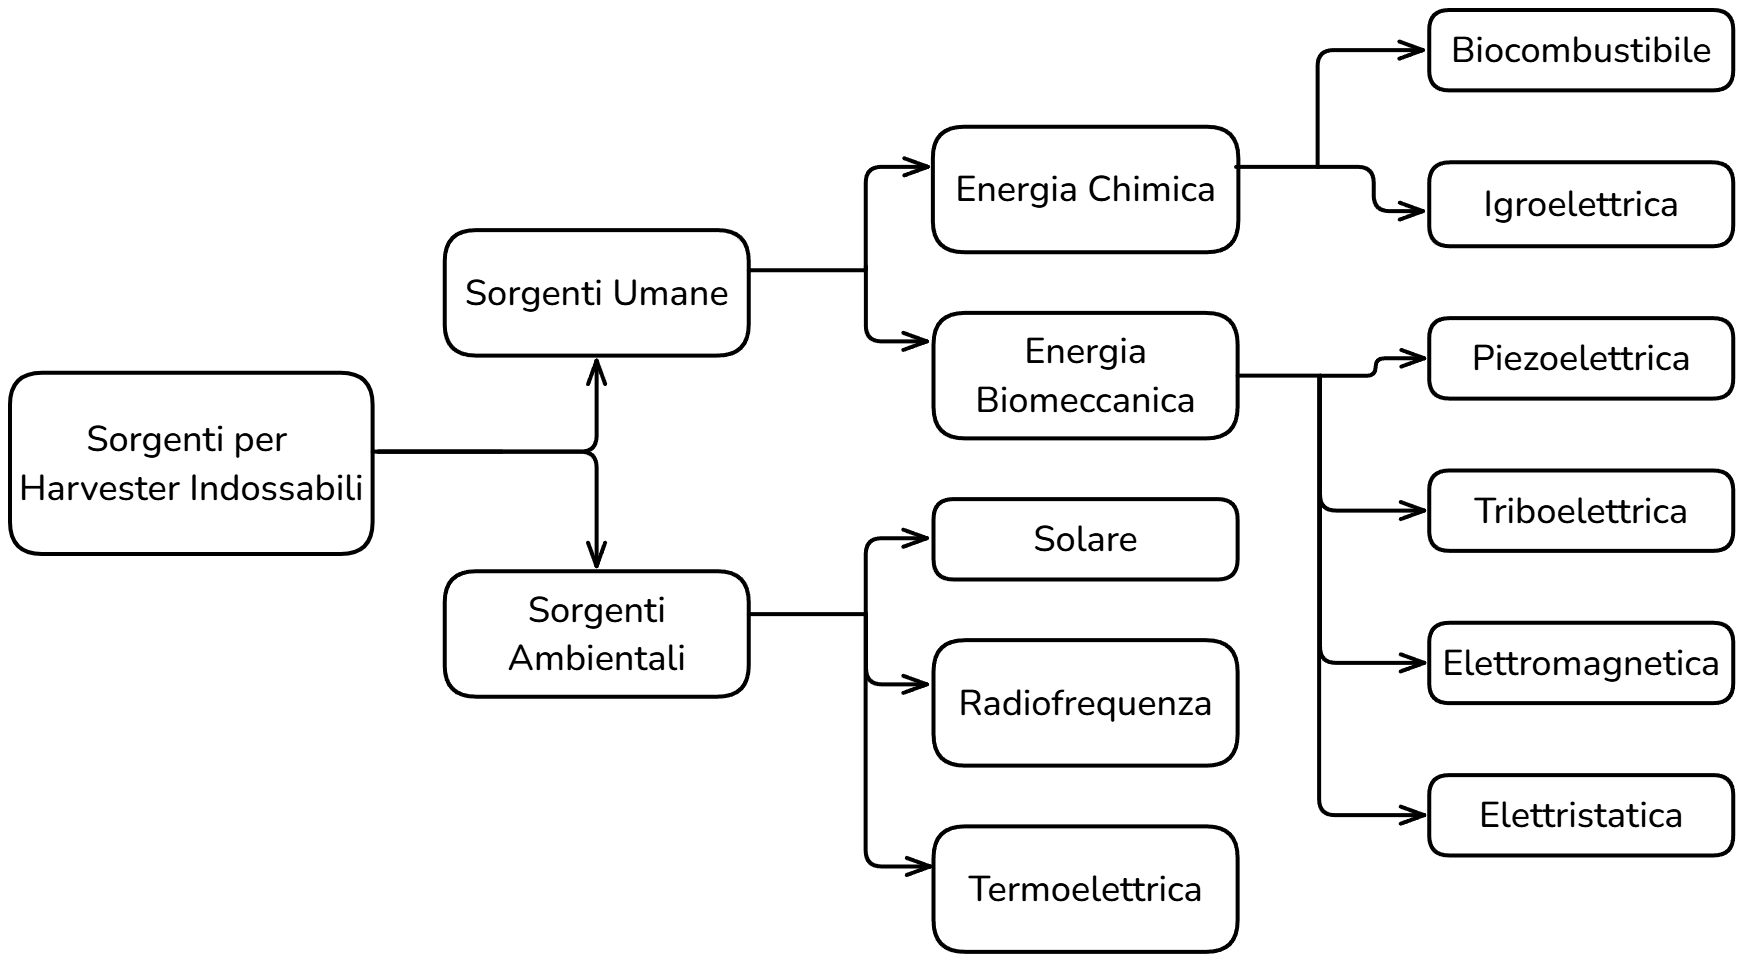
\includegraphics[width=0.9\textwidth]{classificazioni_fonti.png}
        \centering
        \caption{Classificazione delle fonti energetiche a cui puo' essere applicato un harvester per dispositivi indossabili.}
        \label{fig:classificazione}
    \end{figure}
    
    La maggior parte delle fonti in figura \ref{fig:classificazione} non e' sempre disponibile e nemmeno prevedibile. E' possibile pero' usare harvester accoppiati a componenti di accumulo come batterie o supercondensatori quando e' richiesta un'alimentazione regolare. Un'alternativa per monitorare segnali a rischio piu' basso e' accendere il dispositivo solo quando l'energia e' disponibile. Similmente per aumentare l'efficienza si possono alimentare i singoli moduli quando diventano necessari. La gestione intelligente dell'energia richiede una power managment unit.
\end{section}

\begin{section}{Apllicazioni Harvester Energetici}
    Esistono versioni indossabili per la misura non invasiva di molti parametri di interesse rilevante come ECG, EEG, pressione sanguigna, saturazione di ossigeno nel sangue e frequenza respiratoria. Altri dispositivi sono in grado di raccogliere in maniera piu' o meno invasiva fluidi corporei come sangue, sudore o liquido interstiziale per intercettare problemi metabolici. Oltre a raccogliere dati, questi apparati medici possono anche partecipare attivamente alla cura, come nel caso di dosatori di medicinali, elettrostimolatori neuronali o muscolari, pacemaker e defibrillatori impiantabili.
    
    Monitorare facilmente e con costanza questi parametri consente di individuare lo sviluppo di alcune malattie in anticipo rispetto ai metodi tradizionali, aumentando le probabilita' di successo nel trattamento. Nonostante questo, nessun dispositivo medico indossabile commercializzato fa uso di energy harvesting. La ricerca recente ha pero' dimostrato con esempi pratici l'efficacia di questa metodologia. Per dispositivi ad uso esterno facilmente testabili, ma anche per impianti in vivo su animale. Alcuni esempi recenti sono: \begin{itemize}
        \item Un dispositivo in grado di misurare glicemia dal sudore, temperatura e HRV e' stato sviluppato in \cite{mirlouContinuousGlycemicMonitoring2024}. Un harvester RF ne permette il funzionamento continuativo, supportando la batteria.
        \item Per trattare la miopia con esposizione graduale ai farmaci, in \cite{jiangSelfgeneratedElectricitydrivenDrug2024} e' stata sviluppato un dosatore a forma di lente a contatto. La funzione di rilascio e' automatizzata da un nanogeneratore piezoelettrico attivato dal battito delle palpebre.
        \item Un modulo autosufficiente che monitora respiri e temperatura e' stato integrato in mascherine sanitarie in \cite{lanHighefficientIntelligentAntibacterial2024}. In \cite{simInstantDisinfectingFace}, un harvester tribolettrico e' usato per creare un campo elettrico forte abbastanza da disinfettare le maschere.
        \item In \cite{anVivoFlexibleEnergy2024} viene dimostrato l'uso di un harvester piezoelettrico impiantato su tessuto cardiaco porcino.
    \end{itemize}
 
    Soluzioni con harvester hanno alcuni svantaggi rispetto a sola batteria. Tra questi, la bassa densita' energetica e l'affidabilita' incerta li rendono un opzione immatura per scopi medici critici. Questi sono gravosi soprattutto per dispositivi impiantabili che richiedono dimensioni minime e la certezza del funzionamento a lungo termine. I costi di produzione sono alti, dovuti anche alla mancanza di una catena manufatturiera paragonabile a prodotti altamenti diffusi come le batterie.

    E' giusto menzionare che e' possibile applicare l'idea di energy harvester anche a dispositivi non mobili. In questo caso, naturalmente, non si puo' piu' attingere alle fonti energetiche del corpo umano, ma se ne hanno altre come vento o vibrazioni. Un'applicazione di interesse e' usarli per recuperare l'energia di scarto da sistemi piu' grandi come macchinari industriali o mezzi di trasporto. In zone dove e' necessario fare monitoraggi, ma manca distribuzione elettrica anche possono essere una soluzione. Questo permetterebbe di azionare una rete distribuita di sensori o attuatori autonomi. Harvester impegati in questo modo hanno meno restrizioni su dimensioni e affidabilita'. Alcuni esempi recenti sono: \begin{itemize}
        \item Monitoraggio della sicurezza e stato dei mezzi di trasporto come treni o auto trasformando l'energia delle vibrazioni \cite{liSmartRailwayTransportation, liuCompactHybridizedTriboelectricelectromagnetic2024}
        \item Una rete di generatori galleggianti che raccolgono l'energia meccanica delle onde per deionizzare l'acqua marina in loco \cite{renWavepoweredCapacitiveDeionization2024}. 
        \item Sensori per verificare lo stato di macchinari industriali, sfruttandone le vibrazioni \cite{alvarezruedaVibrationEnergyHarvesting2024, gaoHybridGeneratorEfficient2024}, o il calore \cite{deoliveiraDevelopmentHybridEnergy2024}.
    \end{itemize}
    
\end{section}


\include{capitoli/Metodi}

\chapter{Esempio}
    Si sceglie come esempio \cite{kouWearableAllFabricHybrid2024} che offre una realizzazione pratica di un harvester ibrido. L'obbiettivo di questo generatore e' proporre un dispostivo riproducibile in scala e facilmente integrabile nel vestiario. Per fare questo usa una struttura interamente fondata su una base di tessuto e accoppia un generatore triboelettrico a uno RF. Un tessuto elettricamente conduttivo disponibile sul mercato e' usato per realizzare le connessioni su ambo i lati di uno strato di tessuto comune di cotone. In questo modo l'harvester diventa altamente flessibile e facilmente ingrabile in capi di abbigliamento. Avere 2 fonti distinte aumenta le probabilita' che il dispositvo sia sempre in funzione, inoltre queste in particolare si prestano a un design planare.
    
    \begin{figure}[H]
        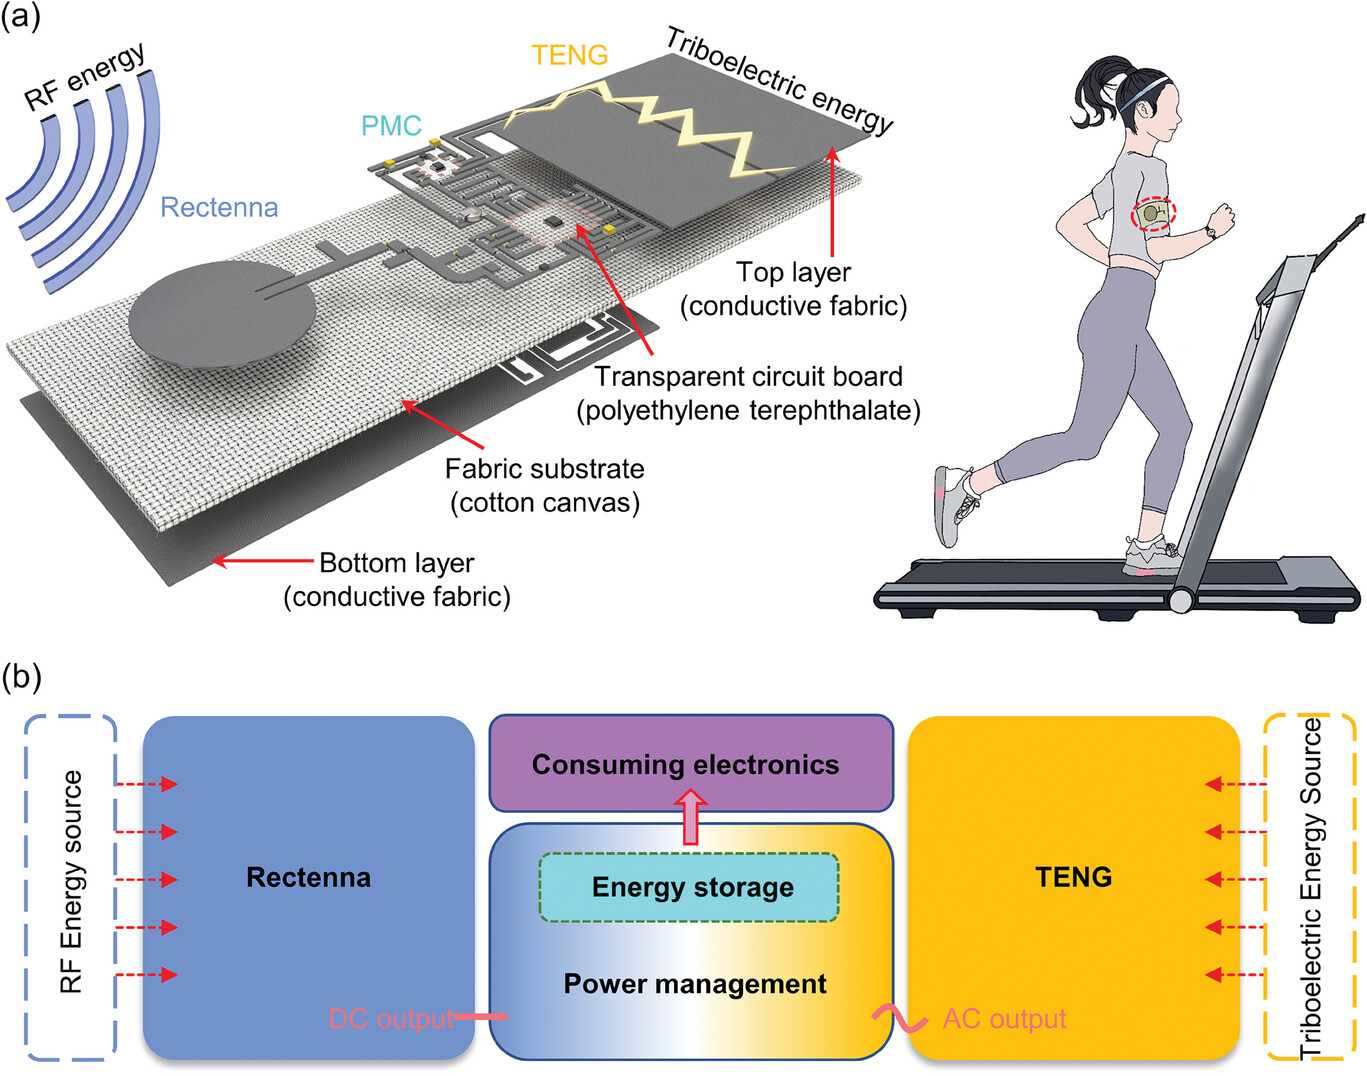
\includegraphics[width=0.8\textwidth]{schema.jpg}
        \centering
        \caption{a) Modello della struttura dell'harvester preso in esempio. b) Schema del funzionamento generale dell'harvester.\cite{kouWearableAllFabricHybrid2024}}
        \label{fig:schema}
    \end{figure}

\begin{section}{Generatori}
    \begin{subsection}{Generatore Triboelettrico}
        In generale i generatori di questo tipo sfruttano la capacita' di alcuni materiali di trasferire carica al contatto. La struttura e' formata da uno strato di propilene fluorato (FEP) libero di scorrere sopra ai due elettrodi di tessuto connettivo che doppiano da secondo materiale triboelettrico. Questa forma detta a scorrimento libero, oltre ad avere un fattore di forma piu' vantaggioso, genera anche piu' energia rispetto al semplice contatto \cite{fuAchievingUltraDurabilityHigh2024}. 
        \begin{figure}[H]
            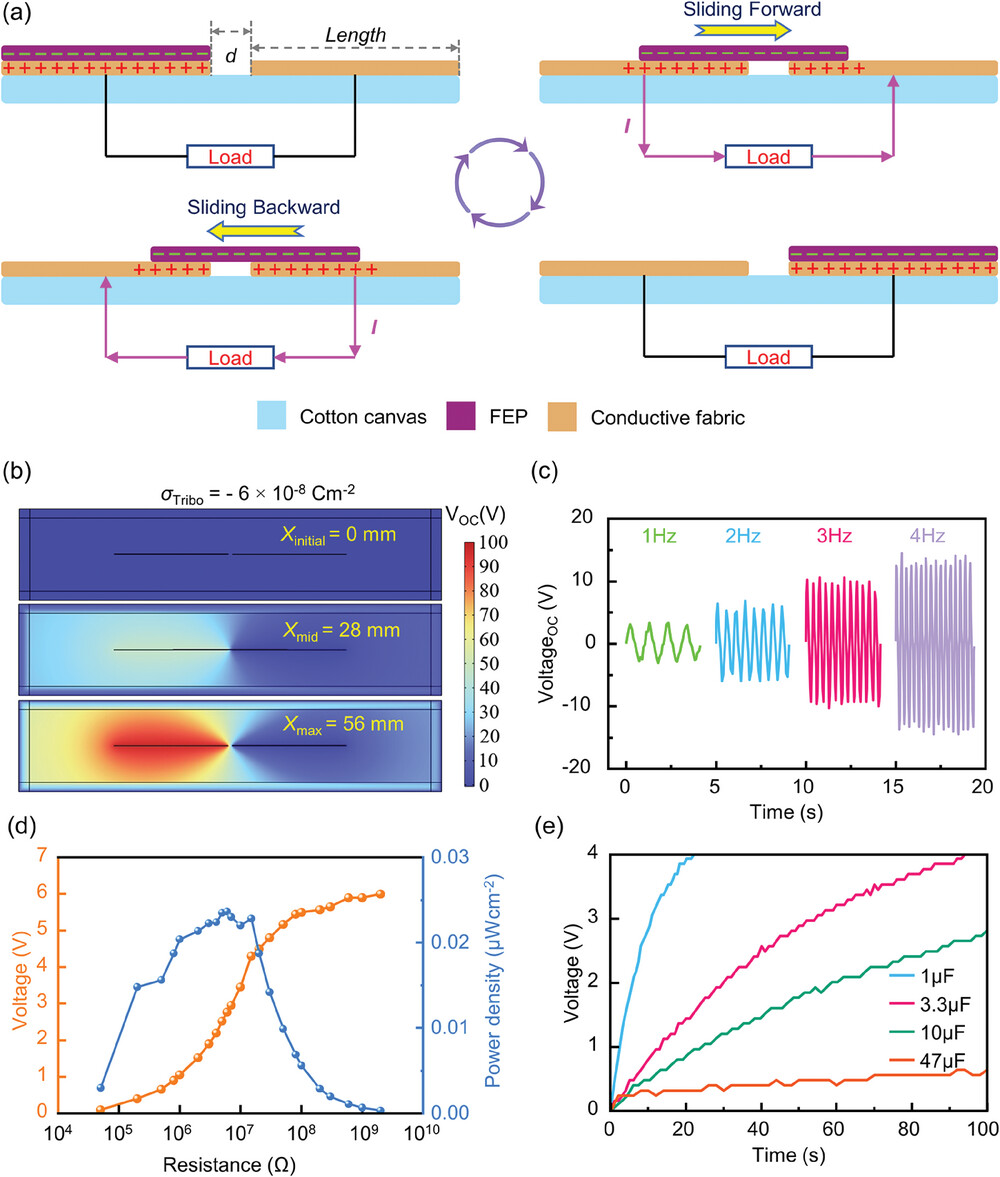
\includegraphics[width=0.8\textwidth]{funzioneTEG.jpg}
            \centering
            \caption{a) Schema del funzionamento del generatore triboelettrico. b) Potenziali simulati a spostamento iniziale, medio e massimo. c) Uscita in tensione a diverse frequenze di scorrimento. d) Dipendenza della tensione e potenza prodotte dal carico. e) Tempi di carica di condensatori commerciali.\cite{kouWearableAllFabricHybrid2024}}
            \label{fig:funzioneTEG}
        \end{figure}
        Il design aperto e i limiti di peso non permettono di ottimizzare altri aspetti che influenzano l'efficienza, come l'umidita' o la pressione tra gli elementi. La tensione massima ottenibile tra gli elettrodi e' determinata dalla densita' di carica ottenibile dal contatto dei materiali. Lo stimolo meccanico genera nello strato libero un movimento oscillatorio e quindi una corrente alternata sul circuito che necessita raddrizzamento. La densita' di potenza massima e' \(0.024\mu Wcm^{-2}\) stata misurata collegando un potenziometro e azionando il movimento a \(2Hz\) per simulare il cammino. Per quanto questo dimostri che il dispositivo e' in grado di raccogliere energia dal movimento umano, la densita' di potenza e' molto bassa se paragonata a una batteria tradizionale, ma anche ai requisiti correnti di dispositivi medici indossabili \cite{gaoAdvancedEnergyHarvesters2024}. Il funzionamento e i risultati sperimentali sono raccolti in figura \ref{fig:funzioneTEG}.
        
    \end{subsection}
    
    \begin{subsection}{Generatore a Radiofrequenza}
        Per raccogliere energia dalle radiazioni presenti nell'ambiente e' stato scelto un harvester con antenna dimensionata per la sola banda attorno ai \(2.45GHz\) usata per connessioni a corto raggio come Wi-Fi e Bluetooth. La distribuzione di onde radio dovute alle comunicazioni elettroniche e' naturalmente concentrata nelle zone urbane. In aree extraurbane la densita' di potenza dovuta a comunicazioni ad ampio raggio scende vistosamente \cite{ibrahimRadioFrequencyEnergy2022}, la scelta di una banda comunemente usata da dispositivi generalmente vicini all'uomo ha quindi il vantaggio di essere piu' consistente nel tempo. La configurazione per l'antenna e' a patch circolare e le dimensioni ottimali per la risonanza sono stati ottenuti attraverso simulazione. Il valore di specific absorbtion rate (SAR) e' un parametro usato per determinare la potenza assorbita da un'unita' di massa di tessuto corporeo \cite{vallozzi26LatestDevelopments2016}. Secondo le simulazioni il SAR e' \(0.073\frac{W}{Kg}\), ben inferiore ai \(2.0\frac{W}{Kg}\) stabiliti dalle norme europee per antenne mobili. In questo caso il SAR e' usato come parametro di efficienza rispetto alla quantita' di radiazione persa dall'antenna nel corpo. 


        {\color{red}
        Un analizzatore (Keysight N5227B) e' usato per misurare la return loss in condizioni libera e a contatto col corpo. Per le dimensioni scelte si nota effettivamente un picco di \(-10\mathrm{dB}\) nel centro banda desiderato e anche quando l'antenna e' indossata lo stesso picco trasla di solo \(20\mathrm{MHz}\).
        La return loss e' generalmente definita come 
        \begin{equation*}
            \begin{aligned}
            RL&=10\log_{10}\left( \frac{P_{in}}{P_{ref}} \right) \mathrm{dB}\\
            RL&=-20\log_{10}\left|\Gamma\right|\mathrm{dB} \textrm{ , dove }\Gamma=\frac{Z_{out}-Z_{in}}{Z_{in}+Z_{out}}\hspace{2em} \textrm{e' il coefficiente di riflessione}
            \end{aligned}
        \end{equation*}
        Questo articolo la usa come una valutazione dell'abbinamento delle impedenze in ingresso e uscita all'antenna, ma il valore ottenuto di\(-10\mathrm{dB}\) e' negativo e indicherebbe una potenza riflessa maggiore delle catturata. Si assume quindi che il valore realmente graficato sia quello del coefficiente di riflessione, che e' spesso sostituito alla return loss \cite{birdDefinitionMisuseReturn2009}. Cio' non detrae pero' dalla conclusione che l'antenna sviluppata e' adatta a ricevere segnali intorno ai \(2.45GHz\).
        }

        \begin{figure}[hbt!]
            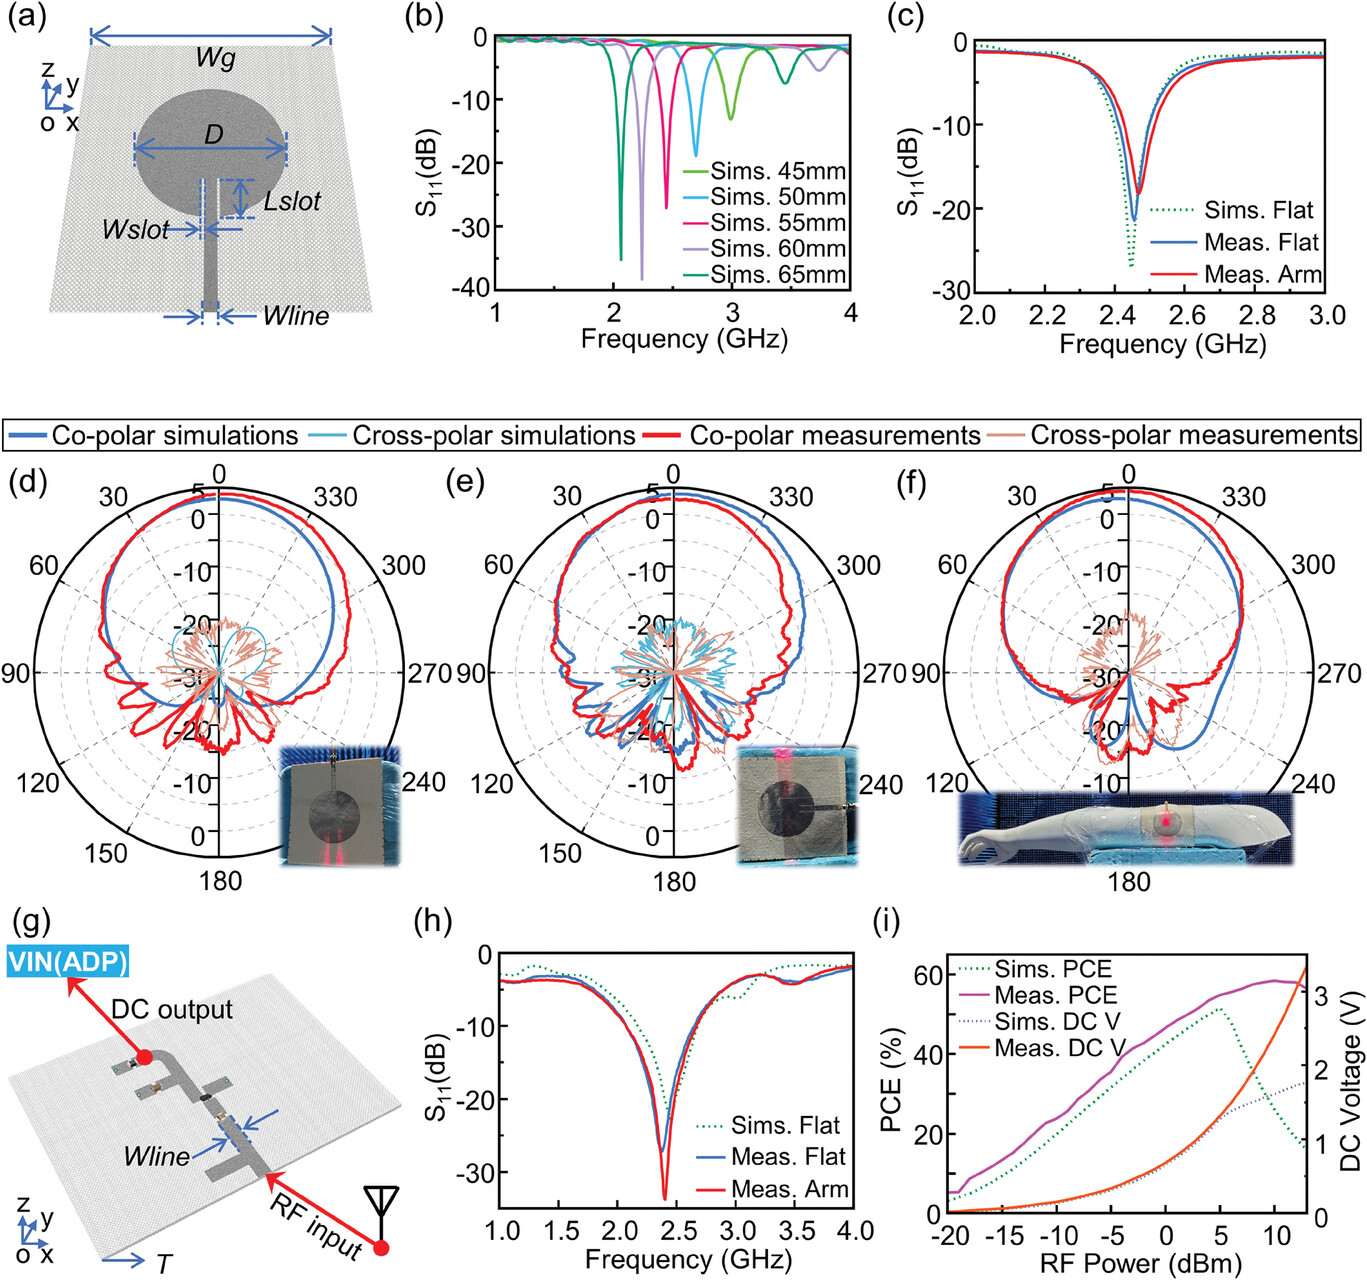
\includegraphics[width=0.8\textwidth]{funzioneRF.jpg}
            \centering
            \caption{a) Struttura dell'antenna. b) Coefficiente di riflessione simulato con diversi diametri. c) Coefficiente di riflessione misurato con antenna piatta e attaccata al corpo. d) Schema di radizione con antenna piatta sul piano xoz. e) Schema di radizione con antenna piatta sul piano xoy. f) Schema di radizione con antenna flessa sul piano xoz. g) Schema della struttura del raddrizzatore. h) Misure e simulazione del coefficiente di riflessione quando l'antenna e' piata o attaccata a un braccio. i) Corrente DC e efficienza di conversione della potenza misurata e simulata rispetto alla potenza in ingresso.\cite{kouWearableAllFabricHybrid2024}}
            \label{fig:funzioneRF}
        \end{figure}
        
        Usando un a camera antieco microonde e' stato graficato lo schema di radiazione in varie posizioni. Lo schema bidimensionale segue le curve dove il guadagno del dispositivo e' massimo. A causa della della configurazione della camera di prova e' stato necessario montare l'antenna su un modello di braccio per caratterizzarne la funzione in flessione. Le misure sono in accordo con le simulazioni e non si presentano particolari differenze nei lobi dovute al cambio di inclinazione o flessione. Quindi si puo' dire che l'antenna e' adatta al funzionamento quando indossata, anche se in posizioni piane come petto e dorso, ma anche dove e' soggetta alla curvatura come in gambe e braccia.

        Un circuito di raddrizzamento per la corrente in uscita dall'antenna e' strettamente necessario per poi caricare la batteria. Il raddrizzatore e' stato progettato per soddisfare alcuni requisiti essenziali. Deve essere flessibile abbastanza da risultare comodamente indossabile. Deve avere massima efficienza di conversione nelle condizioni previste. In fine, e' necessario che le linee conduttive siano dimensionate con precisione, sia la lunghezza che la larghezza influiscono sul buon accoppiamento all'impedenza dell'antenna. Le microstrip di tessuto conduttivo sono tutte larghe \(4.4\mathrm{mm}\), cosi' come la linea in uscita dall'antenna. Si fa uso di un raddrizzatore a doppia semionda, con topologia di Greinacher (\#disegno) per amplificare la tensione prodotta. Vengono installati due condensatri da \(100]\mathrm{pF}\) e due diodi SMS7630-005FL di tipo Schottky, che hanno migliori prestazioni ad alta frequenza e perdite piu' basse rispetto ai diodi a giunzione. Nel circuito raddrizzatore per il generatore triboelettrico, sono stati scelti invece dei diodi (\# dice gli stessi...), piu' efficaci a basse frequenze. Separando il raddrizzatore dal PMG (power managment circuit), la coppia antenna/raddrizzatore diventa un modulo facilmente integrabile in altri dispositivi. La capacita' del modulo di convertire un potenza in ingresso sotto forma RF in DC e' stata valutata inserendo un resistore da \(1\mathrm{K\Omega}\) come carico. La fonte RF e' stata creata usando un generatore di onde (SG-3000PRO) a vari livelli di potenza. L'efficienza di conversione in potenza e' stato determinato misurando la tensione ai capi del carico. 
        \begin{equation*}
            PCE = \frac{P_{carico}}{P_{RF}} = \frac{V_{carico}}{R_{carico}^2P_{RF}}
        \end{equation*}
        I risultati sono graficati in figura \ref{fig:funzioneRF} e mostrano un picco del \(58\%\) nell'efficienza di conversione con \(10\mathrm{dBmW}\) in ingresso, che e' un valore comune nell'intervallo di potenze usate nelle cominicazioni wireless tra dispositivi mobili. 
    \end{subsection}
\end{section}

\begin{section}{Integrazione}
    I due generatori hanno impedenze incompatibili in uscita, sono infatti tre ordini di grandezza distanti\#. Si sviluppa un PMC per convogliare l'energia prodotta dai due in una singola batteria. Il PMC in questo caso deve svolgere le funzioni di: maximum power point tracking (MPPT), undervoltage lockout (UVLO) e protezione di carica. Due microprocessori (ADP5091 e LTC3588), configurati come in figura \ref{fig:schemaPMC}, gestiscono tutte le funzioni. Sono entrambi progettati per applicazioni a bassa potenza e non richiedono alimentazioni oltre quella prodotta dall'harvester stesso. Il ADP5091 e' usato per gestire l'output del generatore RF e proteggere la batteria. In particolare l'uscita REG\_OUT dell'ADP offre la tensione di uscita per il dispositivo da collegare all'harvester quando il componente di accumulo ha raggiunto la tensione minima. Il LTC3588 e' usato per gestire l'output del generatore triboelettrico. Un raddrizzatore ad alta efficienza per alte frequenze e' integrato  tra i pin di ingresso, questo funziona anche da blocco per flussi di corrente verso il TEG.

    \begin{figure}[hbt!]
        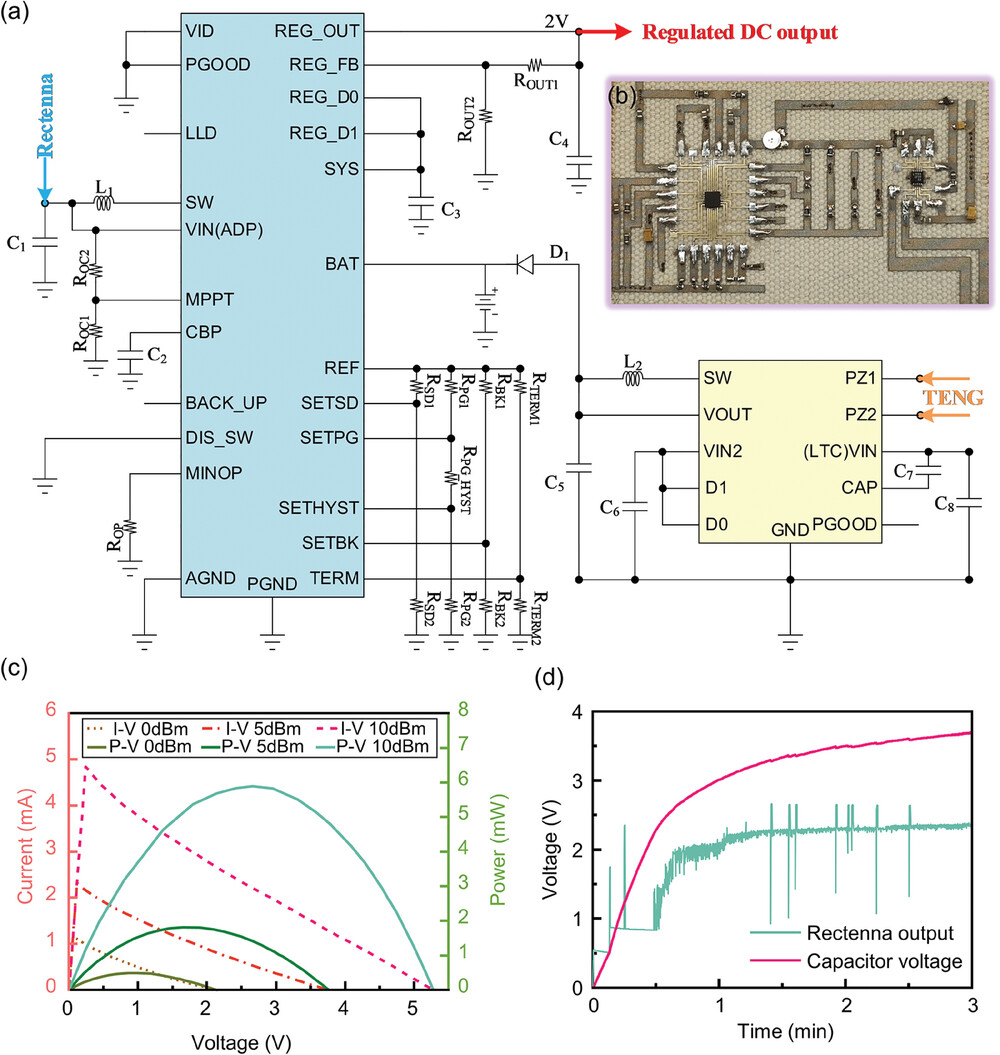
\includegraphics[width=0.9\textwidth]{schemaPMC.jpg}
        \centering
        \caption{a) Schema circuitale del PMC. b) Vista dall'alto del PMC assemblato sul tessuto. c) Dipendenza di corrente e potenza dalla tensione all'uscita del raddrizzatore, per diversi livelli di potenza in ingresso. d) Crescita del potenziale misurata in fase di carica.\cite{kouWearableAllFabricHybrid2024}}
        \label{fig:schemaPMC}
    \end{figure}

    \begin{subsection}{MPPT}
        Le tecniche di MPPT cercano di ottimizzare la potenza convertita da un generatore modificando l'impedenza del circuito, in modo da ottenere il massimo prodotto tra tensione e corrente. Il metodo di MPPT e' fractional open circuit voltage (FOCV), come descritto nel datasheet del ADP5091 \cite{ADP5091DatasheetProduct}. Il metodo FOCV e' comunemente usato in campo fotovoltaico, ma il funzionamento del modulo antenna e raddrizzatore e' paragonabile.L'uscita in tensione varia poco all'interno della banda di frequenze interessata, ma varia considerevolemte con l'incidenza delle onde. La tensione in condizione di circuito aperto varia al variare dell'incidenza di onde RF, la MCU ne prende periodicamente un campione, salvandola in un condensatore. La tensione di massima potenza e' calcolata secondo:
        \begin{equation*}
            V_{MPPT} = V_{IN}\underbrace{\left(\frac{R_{OC1}}{R_{OC1}+R_{OC2}}\right)}_\mathrm{k}
         \end{equation*}
        Il processore cambia poi l'impedenza di ingresso alla porta VIN a cui e' collegato il raddrizzatore in modo da ottenere la tensione ottimale. Il fattore moltiplicativo dato dalle resistenze e' stato determinato sperimentalmente usando una resistenza programmabile mentre l'harvester era sottoposto a diversi livello di irradiazione (\(0\mathrm{dBmW},5\mathrm{dBmW},10\mathrm{dBmW}\)). Il valore medio del fattore moltiplicativo e' \(0.5\), per cui sono stati installati due resistori \((R_{OC1},R_{OC2})\) uguali da \(10\mathrm{M\Omega}\). Il periodo di campionamento di default e' \(16\mathrm{s}\), mentre il tempo per il campionamento e' \(256\mathrm{ms}\), nessuno dei due e' stato modificato.
    \end{subsection}

    \begin{subsection}{UVLO}
        L'UVLO e' implementato nel controllore LTC3588, che gestisce la produzione del generatore triboelettrico. Un condensatore \((C_8)\) immagazzina preventivamente l'energia in entrata. Quando la tensione su  \(C_8\) supera la soglia scelta per UVLO, viene stabilita una connessione attraverso un convertitore di tensione step-down per caricare \(C_5\). Quest'ultimo condensatore e' collegato alla batteria, e la sua corrente e' direzionata da un diodo. Sia in ingresso che uscita sono stati usati condensatori elettrolitici al tantalio, per via della migliore capacita', efficienza di carica e bassa corrente di dispersione \cite{torkiElectrolyticCapacitorProperties2023}.
    \end{subsection}

    \begin{subsection}{Protezione di Carica}
        Mantere la tensione imposta sulla batteria all'interno di un certo intervallo e' essenziale per ridurne l'usura. La carica massima e' stabilita a \(3.6\mathrm{V}\) attraverso il dimensionemanto delle resistenze \(R_{TERM1}=5.9\mathrm{M\Omega},R_{TERM2}=4.12\mathrm{M\Omega}\), la somma delle resistenze e' sopra ai \(6\mathrm{M\Omega}\), come consigliato dal produttore del MCU per limitare la corrente di quiescenza. Con tensione di riferimento interno \(V_{INT\_REF}=1.011\mathrm{V}\) \#, di default, la tensione massima ammessa sulla batteria e': 
        \begin{equation*}
            V_{BAT_TERM} = \frac{3}{2}V_{INT\_REF}\left(1+\frac{R_{TERM1}}{R_{TERM2}}\right) \approx 3.6V
        \end{equation*}
        \#anche scarica valori in S
    \end{subsection}

    \begin{subsection}{Integrazione}
        L'harvester ibrido e' stato testato in condizioni controllate ed e' stato misurato quanto velocemente carica un supercondesatore da \(1000\mathrm{\mu F}\). La fonte RF e' stata posta a \(12\mathrm{cm}\) e emette \(13\mathrm{dBmW}\), mentre il movimento e' azionato da un attutatore lineare a \(2\mathrm{Hz}\). In queste condizioni il condensatore supera di poco la tensione massima stabilita e resta stabile a \(3.7\mathrm{V}\) dopo \(3\mathrm{m}\). Si ottiene una potenza media di \(38\mathrm{\mu W}\), con picco \(111\mathrm{\mu W}\), che alle dimensioni di \(10\mathrm{cm}\times30\mathrm{cm}\) corrisponde a \(0.13\mathrm{\mu W}\) medi. Per verificarne l'applicabilita' ad un caso pratico, l'harvester e' stato indossato da un volontario e collegato a due dispositivi di cui e' stato misurato il tempo di funzionamento. Un sensore di temperatura commercialeha portato il condensatore da \(3.65\mathrm{V}\) alla sua tensione di funzionamento minima \(1.5\mathrm{V}\) in \(42\mathrm{2}\).
        I tempi di carica dei generatori singoli e la modalita' ibrida sono stati raccolti in un grafico in figura \ref{fig:risultati}. Da qui si puo' notare come la potenza generata dalla parte triboelettrica sia trascurabile rispetto a quella generata dall'antenna.

        \begin{figure}{H}
            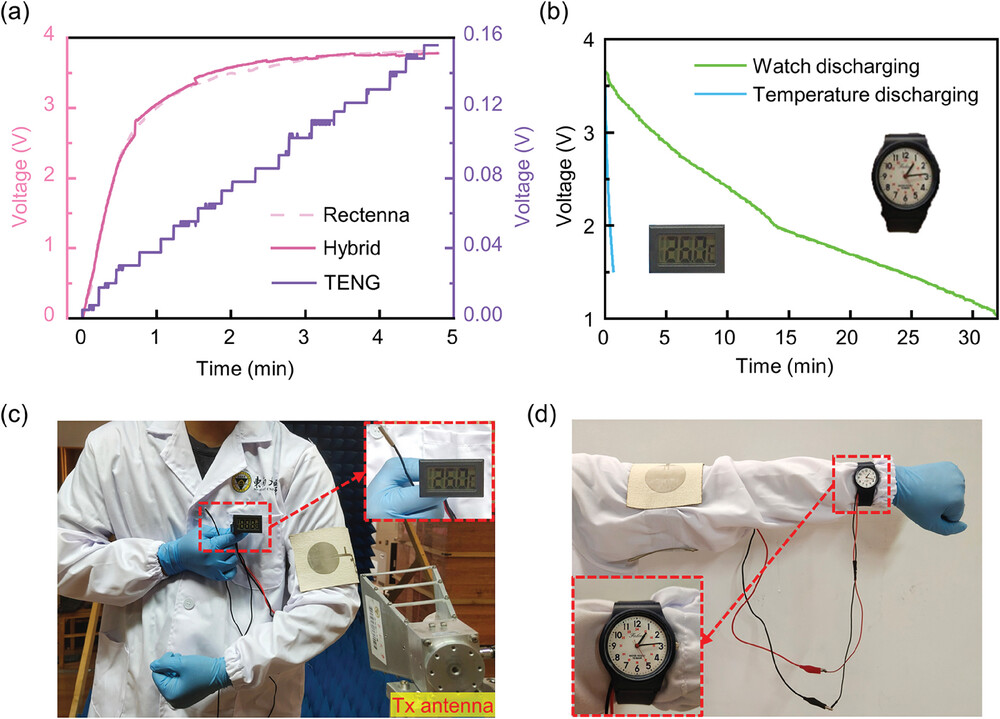
\includegraphics[width=0.85\textwidth]{risultati.jpg}
            \centering
            \caption{a) Tempi di carica singoli e modalita' ibrida. b) Tempi di funzionamento dispositivi reali. c) Configurazione sensore di temperatura. d) Configurazione orologio. \cite{kouWearableAllFabricHybrid2024}}
            \label{fig:risultati}
        \end{figure}

        In questo caso il funzionamento ibrido e' svantaggioso, in quanto la densita' di potenza aumenterebbe se il dispositivo fosse limitato a una fonte RF. Essendo un harvester sviluppato per uso esterno avvolto ad un arto, diminuire ulteriormente le dimensioni sul piano non e' particolarmente vantaggioso. Per cui, avere il basso flusso energetico raccolto dal movimento potrebbe essere comunque vantaggioso, in particolare vista la possibilita' di produrlo in modo semplice. Andrebbero pero' considerate alternative come fotovoltaico o termoelettrico, che nella stessa posizione non si trovano in condizioni di bassa efficienza come il triboelettrico. 
    \end{subsection}

    \# potrei guardare simulazioni o produzione su tessuto

\end{section}

\begin{chapter}{Conclusione}
    In questa tesi \'e stata studiata la possibilit\'a di alimentare dispositivi indossabili attraverso generatori integrati a essi, detti energy harvester. Tecnologie di questo tipo attingono a fonti energetiche esterne al dispositivo che alimentano. Le fonti considerate sono sostenibili e a bassa intensit\'a, ma generalmente presenti attorno all'uomo. L'obbiettivo principale \'e sostituire o supportare le batterie comunemente usate. Questo renderebbe i dispositivi mobili meglio capaci di operare in modo ininterrotto, con meno manutenzione e quindi anche in luoghi isolati dalla distribuzione elettrica. I vantaggi dell'energy harvesting sono interessanti per applicazioni IoT, ma ancora di pi\'u per dispositivi medici indossabili e impiantabili. Restrizioni sulle dimensioni e la necessit\'a di avere alta efficienza sono i principali ostacoli all'uso allargato di energy harvesting.

    Si \'e scelto come esempio un harvester ibrido che converte segnali intorno ai \(2.5\mathrm{GHz}\) dovuti alle comunicazioni wireless e le vibrazioni dovute al movimento umano. Viene dimostrato che la potenza prodotta da questo \'e sufficiente ad alimentare dispositivi a bassa potenza. Il fatto di essere altamente flessibile e interamente costruito su substrato tessile permette l'integrazione nel vestiario e quindi la connessione a vari tipi di dispositivi indossabili.  
\end{chapter}


%biblio
\bibliographystyle{unsrt}
\bibliography{test}


\end{document}